\documentclass[12pt,a4paper]{article}
\usepackage[utf8]{inputenc}
\usepackage[T1]{fontenc}
\usepackage{amsmath}
\usepackage{amsfonts}
\usepackage{amssymb}
\usepackage{graphicx}
\usepackage{hyperref}
\usepackage[polish]{babel}
\usepackage{algorithm}
\usepackage{algpseudocode}
\usepackage{booktabs}
\usepackage{float}
\usepackage{subcaption}
\usepackage{changepage}
\usepackage{geometry}
\usepackage{xcolor}

% Marginesy
\geometry{a4paper, margin=2.5cm}

% Fix for Polish algorithm name
\makeatletter
\def\ALG@name{Algorytm}
\makeatother

% Make font smaller in algorithm listings
\makeatletter
\algrenewcommand\ALG@beginalgorithmic{\footnotesize}
\makeatother

\title{Analiza Globalnej Wypukłości oraz Projekt Ulepszonego Algorytmu Hybrydowego dla Problemu Dwóch Komiwojażerów}
\author{Filip Rosiak 151799  \and Eryk Stec 152948}
\date{\today}

\begin{document}

\maketitle

\begin{abstract}
Praca prezentuje wyniki dwóch etapów badań nad problemem komiwojażera z dwoma rozłącznymi cyklami (2-TSP). W pierwszym etapie (Laboratorium 6) przeprowadzono analizę globalnej wypukłości krajobrazu przeszukiwania dla instancji \texttt{kroa200} i \texttt{krob200}. Wykorzystano dwie miary podobieństwa rozwiązań: liczbę par wierzchołków przydzielonych do tego samego cyklu oraz liczbę wspólnych krawędzi. Analiza wykazała korelacje między kosztem rozwiązania a jego podobieństwem do znanego, dobrego rozwiązania oraz do innych optimów lokalnych, dostarczając wglądu w strukturę przestrzeni rozwiązań.

W drugim etapie (Laboratorium 7) skupiono się na zaprojektowaniu i implementacji ulepszonego algorytmu hybrydowego, nazwanego `EnhancedHaeOrOpt`. Algorytm ten rozbudowuje standardowy algorytm ewolucyjny (HAE) poprzez wprowadzenie zróżnicowanej inicjalizacji populacji, zaawansowanej rekombinacji, mechanizmów dywersyfikacji i elitaryzmu, oraz – co kluczowe – adaptacyjnego przeszukiwania lokalnego (ALS). ALS dynamicznie wybiera między operatorem wymiany krawędzi (EdgeExchange) a operatorem Or-Opt. Testy na instancjach \texttt{kroa200} i \texttt{krob200}, uśrednione z 20 uruchomień, wykazały, że `EnhancedHaeOrOpt` osiąga istotną poprawę jakości rozwiązań w porównaniu do bazowej wersji HAE (poprawa średnio +1.51\% dla \texttt{kroa200} i +2.41\% dla \texttt{krob200}).
\end{abstract}

\section{Opis Problemu}
Rozważany problem jest modyfikacją klasycznego problemu komiwojażera. Dany jest zbiór wierzchołków i symetryczna macierz odległości pomiędzy dowolną parą wierzchołków. Zadanie polega na ułożeniu dwóch rozłącznych zamkniętych ścieżek (cykli), każda zawierająca 50\% wierzchołków (jeżeli liczba wierzchołków w instancji nie jest parzysta, to pierwsza ścieżka zawiera jeden wierzchołek więcej), minimalizując łączną długość obu ścieżek.

Do testów wykorzystano instancje \texttt{kroa200} i \texttt{krob200} z biblioteki TSPLib. Są to dwuwymiarowe instancje euklidesowe, gdzie dla każdego wierzchołka podane są dwie współrzędne, a odległość pomiędzy wierzchołkami jest odległością euklidesową zaokrąglaną do liczby całkowitej.

\section{Laboratorium 6: Analiza Globalnej Wypukłości Krajobrazu Przeszukiwania}
\label{sec:lab6}

\subsection{Cel Zadania}
Celem tego etapu było zbadanie struktury krajobrazu przeszukiwania dla problemu 2-TSP na wybranych instancjach. Analiza globalnej wypukłości pozwala ocenić, czy lepsze rozwiązania są do siebie bardziej podobne i czy tworzą pewnego rodzaju "lejek" prowadzący do globalnego optimum. Zrozumienie tej struktury może pomóc w projektowaniu bardziej efektywnych algorytmów metaheurystycznych.

\subsection{Metodyka}
Analizę przeprowadzono zgodnie z wytycznymi zadania:
\begin{enumerate}
    \item Dla każdej instancji (\texttt{kroa200}, \texttt{krob200}) wygenerowano 1000 losowych optimów lokalnych. Każde optimum lokalne uzyskano startując z losowego rozwiązania początkowego i stosując algorytm lokalnego przeszukiwania (LS) w wersji Candidate Steepest (k=10) z sąsiedztwem Edge Exchange, aż do osiągnięcia lokalnego minimum.
    \item Wygenerowano również jedno "bardzo dobre rozwiązanie" referencyjne ($S_{best}$) dla każdej instancji, używając najlepszej dostępnej metody z wcześniejszych eksperymentów (np. wielokrotne uruchomienia HAE).
    \item Dla każdego z 1000 losowych optimów lokalnych ($S_i$) obliczono dwie wartości podobieństwa:
    \begin{itemize}
        \item Podobieństwo do $S_{best}$.
        \item Średnie podobieństwo do wszystkich pozostałych $1000-1$ optimów lokalnych ze zbioru.
    \end{itemize}
    \item Zastosowano dwie miary podobieństwa (analizowane oddzielnie):
    \begin{enumerate}
        \item \textbf{Liczba par wierzchołków przydzielonych razem do jednego cyklu (VP):} Dla dwóch rozwiązań $S_a$ i $S_b$, zlicza się, ile par wierzchołków $(u,v)$ znajduje się w tym samym cyklu w $S_a$ ORAZ w tym samym cyklu w $S_b$. Miara ta jest normalizowana przez całkowitą możliwą liczbę par wierzchołków, które mogą być razem w cyklu.
        \item \textbf{Liczba wspólnych krawędzi (CE):} Zlicza się, ile krawędzi $(u,v)$ występuje w obu rozwiązaniach $S_a$ i $S_b$. Miara ta jest normalizowana przez całkowitą liczbę krawędzi w rozwiązaniu (czyli N, liczbę wierzchołków).
    \end{enumerate}
    \item Sporządzono wykresy, gdzie na osi X odłożono wartość funkcji celu (koszt) optimów lokalnych, a na osi Y obliczone wartości podobieństwa (zarówno do $S_{best}$, jak i średnie do pozostałych).
    \item Obliczono współczynnik korelacji Pearsona między kosztem a każdą z miar podobieństwa dla obu typów odniesienia.
\end{enumerate}

\subsection{Wyniki Analizy Globalnej Wypukłości}
Przeprowadzona analiza globalnej wypukłości dla instancji \texttt{kroa200} i \texttt{krob200} obejmowała generowanie 1000 losowych optimów lokalnych dla każdej z nich. Dla każdego optimum lokalnego obliczono jego podobieństwo do rozwiązania referencyjnego ($S_{best}$) oraz średnie podobieństwo do pozostałych 999 optimów lokalnych. Użyto dwóch miar: liczby par wierzchołków w tych samych cyklach (VP) oraz liczby wspólnych krawędzi (CE).

Wyniki współczynników korelacji Pearsona pomiędzy kosztem rozwiązania a miarami podobieństwa przedstawiono poniżej (pełne wyniki znajdują się w pliku \texttt{latex/output/lab6\_correlation\_results.txt}):
\begin{itemize}
    \item Dla instancji \textbf{kroa200}:
    \begin{itemize}
        \item Korelacja (Koszt vs Podobieństwo VP do $S_{best}$): \textbf{-0.0800}
        \item Korelacja (Koszt vs Podobieństwo CE do $S_{best}$): \textbf{-0.4237}
        \item Korelacja (Koszt vs Średnie Podobieństwo VP do Innych): \textbf{-0.4263}
        \item Korelacja (Koszt vs Średnie Podobieństwo CE do Innych): \textbf{-0.6803}
    \end{itemize}
    \item Dla instancji \textbf{krob200}:
    \begin{itemize}
        \item Korelacja (Koszt vs Podobieństwo VP do $S_{best}$): \textbf{-0.0627}
        \item Korelacja (Koszt vs Podobieństwo CE do $S_{best}$): \textbf{-0.3660}
        \item Korelacja (Koszt vs Średnie Podobieństwo VP do Innych): \textbf{-0.4345}
        \item Korelacja (Koszt vs Średnie Podobieństwo CE do Innych): \textbf{-0.6910}
    \end{itemize}
\end{itemize}

Wykresy ilustrujące te zależności przedstawiono na Rysunkach \ref{fig:kroa200_convexity_sbest_plots}, \ref{fig:kroa200_convexity_avg_plots}, \ref{fig:krob200_convexity_sbest_plots} oraz \ref{fig:krob200_convexity_avg_plots}.

\begin{figure}[H]
\begin{adjustwidth}{-1cm}{-1cm}
    \centering
    \begin{subfigure}[b]{0.8\textwidth}
        \centering
        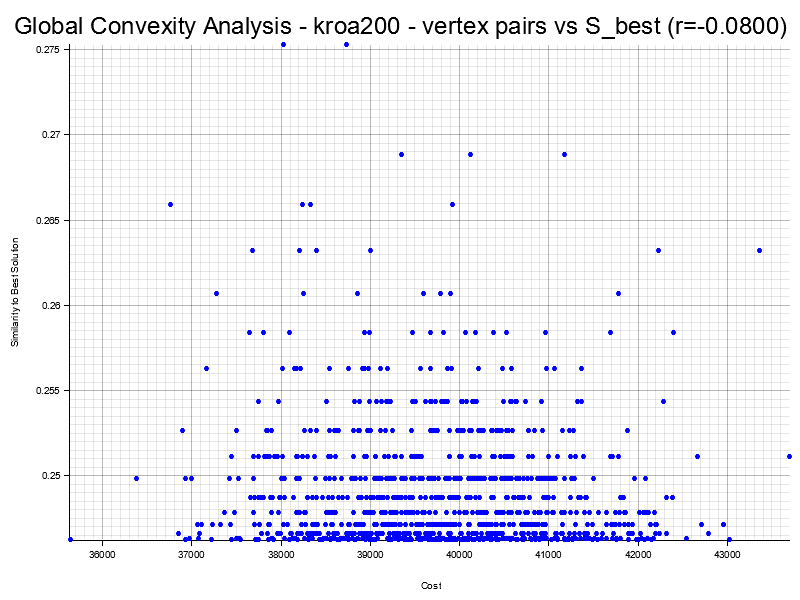
\includegraphics[width=\textwidth]{output/kroa200_convexity_vertex_pairs_s_best.png}
        \caption{kroa200 - Pary Wierzchołków (VP) vs Koszt (do $S_{best}$, r=-0.0800)}
        \label{fig:kroa200_convexity_vp_sbest}
    \end{subfigure}
    \hfill
    \begin{subfigure}[b]{0.8\textwidth}
        \centering
        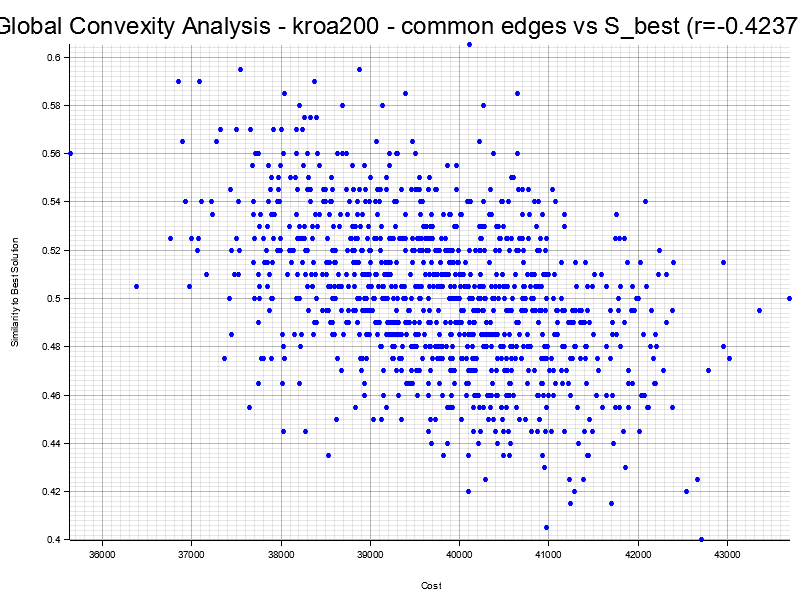
\includegraphics[width=\textwidth]{output/kroa200_convexity_common_edges_s_best.png}
        \caption{kroa200 - Wspólne Krawędzie (CE) vs Koszt (do $S_{best}$, r=-0.4237)}
        \label{fig:kroa200_convexity_ce_sbest}
    \end{subfigure}
    \caption{Wykresy analizy globalnej wypukłości dla instancji kroa200 (Lab 6). Zależność podobieństwa do $S_{best}$ od kosztu.}
    \label{fig:kroa200_convexity_sbest_plots}
\end{adjustwidth}
\end{figure}

\begin{figure}[H]
\begin{adjustwidth}{-1cm}{-1cm}
    \centering
    \begin{subfigure}[b]{0.8\textwidth}
        \centering
        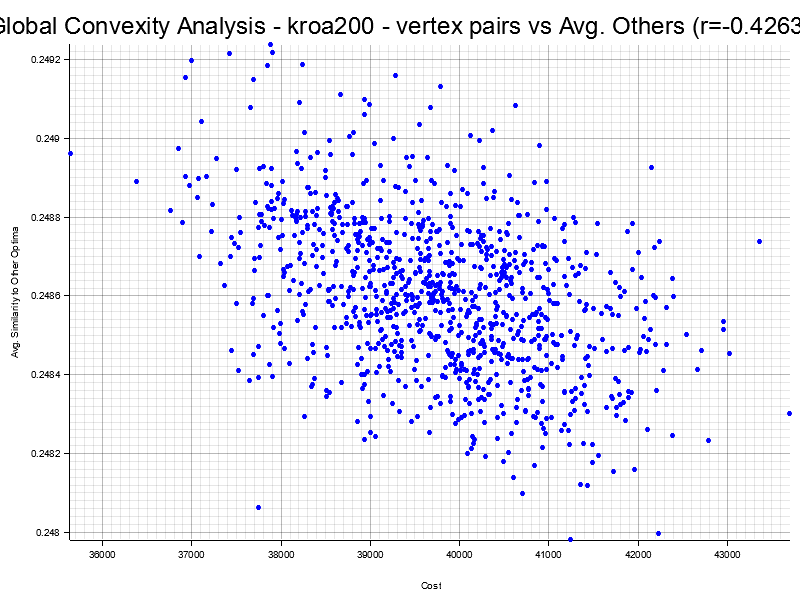
\includegraphics[width=\textwidth]{output/kroa200_convexity_vertex_pairs_avg_others.png}
        \caption{kroa200 - Pary Wierzchołków (VP) vs Koszt (średnie do innych, r=-0.4263)}
        \label{fig:kroa200_convexity_vp_avg}
    \end{subfigure}
    \hfill
    \begin{subfigure}[b]{0.8\textwidth}
        \centering
        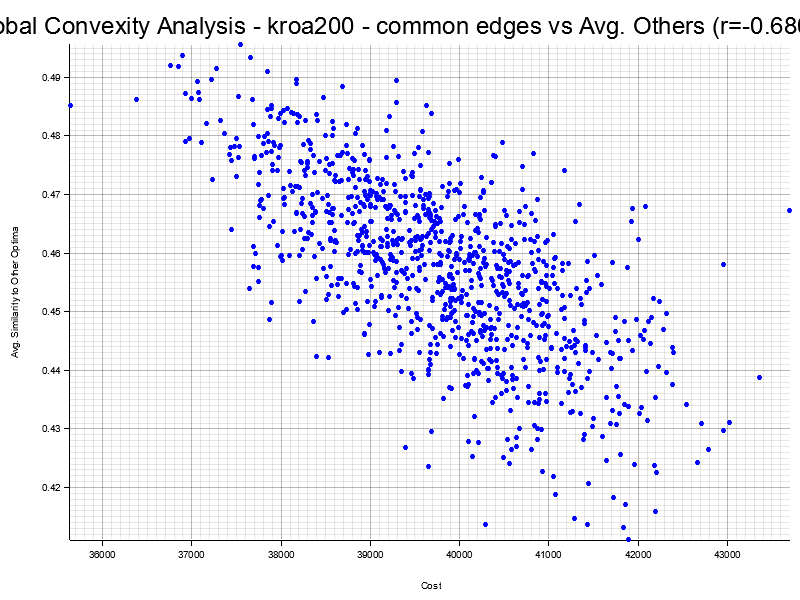
\includegraphics[width=\textwidth]{output/kroa200_convexity_common_edges_avg_others.png}
        \caption{kroa200 - Wspólne Krawędzie (CE) vs Koszt (średnie do innych, r=-0.6803)}
        \label{fig:kroa200_convexity_ce_avg}
    \end{subfigure}
    \caption{Wykresy analizy globalnej wypukłości dla instancji kroa200 (Lab 6). Zależność średniego podobieństwa do innych optimów lokalnych od kosztu.}
    \label{fig:kroa200_convexity_avg_plots}
\end{adjustwidth}
\end{figure}

\begin{figure}[H]
\begin{adjustwidth}{-1cm}{-1cm}
    \centering
    \begin{subfigure}[b]{0.8\textwidth}
        \centering
        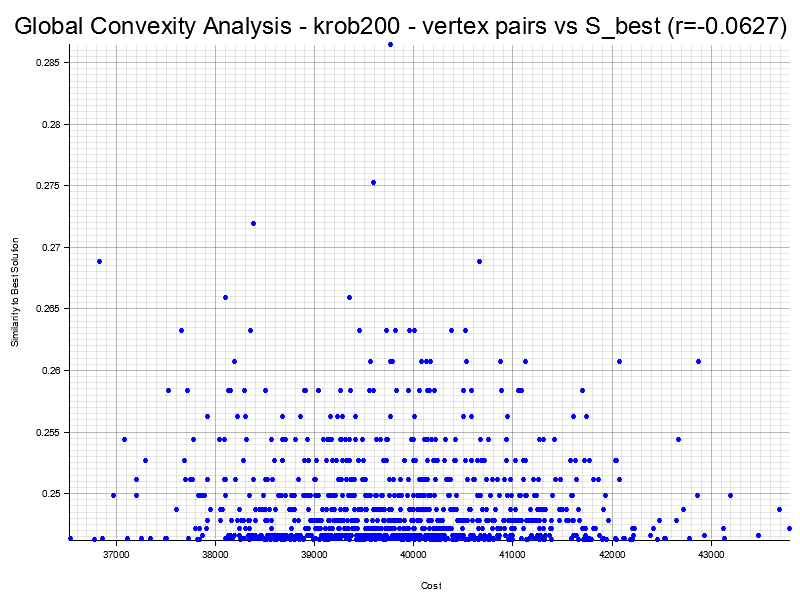
\includegraphics[width=\textwidth]{output/krob200_convexity_vertex_pairs_s_best.png}
        \caption{krob200 - Pary Wierzchołków (VP) vs Koszt (do $S_{best}$, r=-0.0627)}
        \label{fig:krob200_convexity_vp_sbest}
    \end{subfigure}
    \hfill
    \begin{subfigure}[b]{0.8\textwidth}
        \centering
        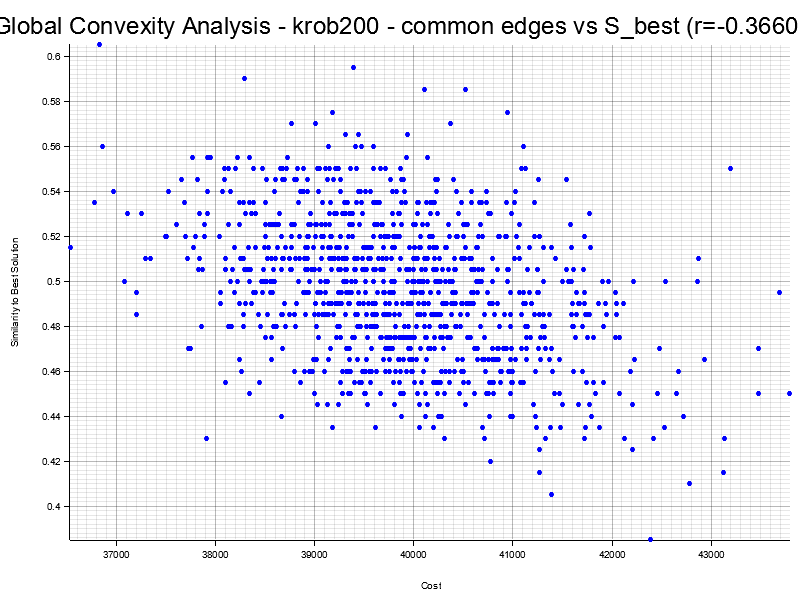
\includegraphics[width=\textwidth]{output/krob200_convexity_common_edges_s_best.png}
        \caption{krob200 - Wspólne Krawędzie (CE) vs Koszt (do $S_{best}$, r=-0.3660)}
        \label{fig:krob200_convexity_ce_sbest}
    \end{subfigure}
    \caption{Wykresy analizy globalnej wypukłości dla instancji krob200 (Lab 6). Zależność podobieństwa do $S_{best}$ od kosztu.}
    \label{fig:krob200_convexity_sbest_plots}
\end{adjustwidth}
\end{figure}

\begin{figure}[H]
\begin{adjustwidth}{-1cm}{-1cm}
    \centering
    \begin{subfigure}[b]{0.8\textwidth}
        \centering
        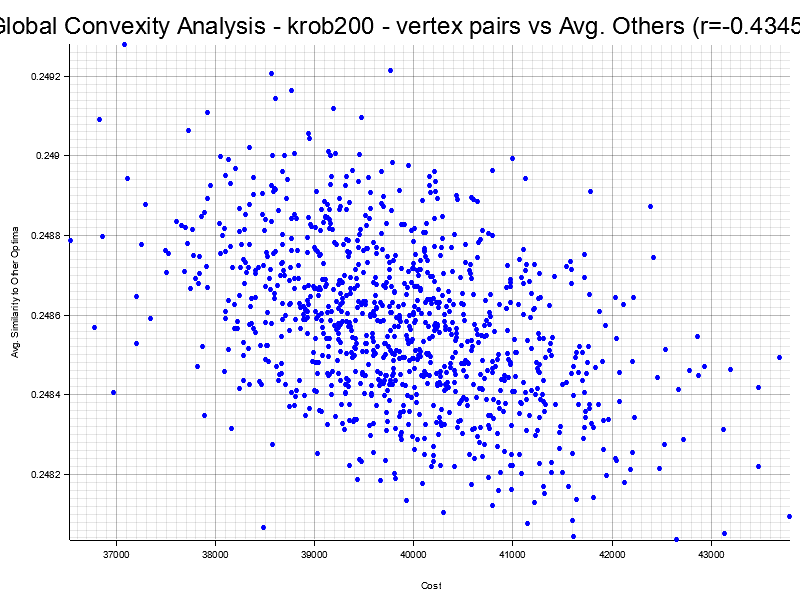
\includegraphics[width=\textwidth]{output/krob200_convexity_vertex_pairs_avg_others.png}
        \caption{krob200 - Pary Wierzchołków (VP) vs Koszt (średnie do innych, r=-0.4345)}
        \label{fig:krob200_convexity_vp_avg}
    \end{subfigure}
    \hfill
    \begin{subfigure}[b]{0.8\textwidth}
        \centering
        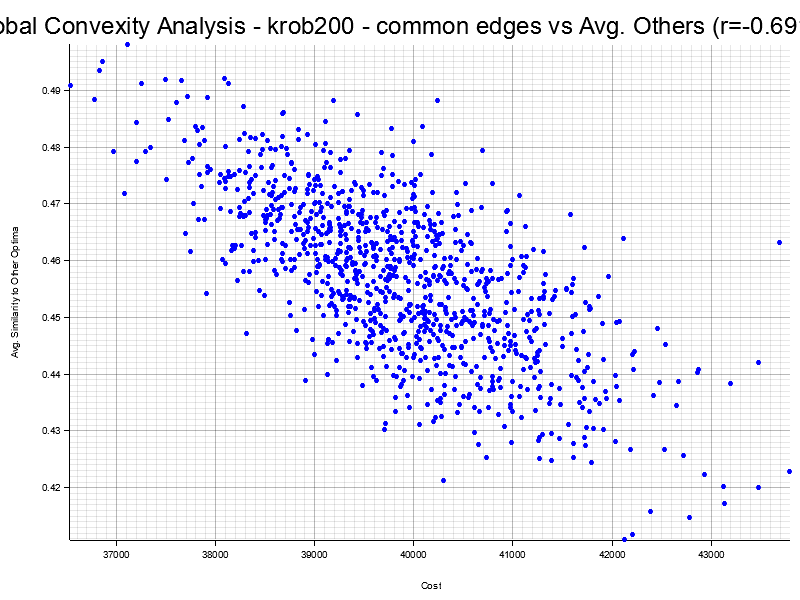
\includegraphics[width=\textwidth]{output/krob200_convexity_common_edges_avg_others.png}
        \caption{krob200 - Wspólne Krawędzie (CE) vs Koszt (średnie do innych, r=-0.6910)}
        \label{fig:krob200_convexity_ce_avg}
    \end{subfigure}
    \caption{Wykresy analizy globalnej wypukłości dla instancji krob200 (Lab 6). Zależność średniego podobieństwa do innych optimów lokalnych od kosztu.}
    \label{fig:krob200_convexity_avg_plots}
\end{adjustwidth}
\end{figure}


\subsection{Wnioski z Laboratorium 6}
Analiza wykresów punktowych oraz współczynników korelacji Pearsona dostarcza istotnych informacji na temat struktury krajobrazu przeszukiwania dla badanych instancji problemu 2-TSP:
\begin{itemize}
    \item \textbf{Silna korelacja dla średniego podobieństwa wspólnych krawędzi (CE):} Najbardziej znaczącym wynikiem jest silna ujemna korelacja między kosztem lokalnego optimum a jego średnim podobieństwem do pozostałych optimów lokalnych, mierzonym liczbą wspólnych krawędzi. Dla instancji \texttt{kroa200} współczynnik ten wynosi r = -0.6803, a dla \texttt{krob200} r = -0.6910. Oznacza to wyraźną tendencję: im niższy (lepszy) koszt ma dane optimum lokalne, tym więcej wspólnych krawędzi dzieli ono przeciętnie z innymi znalezionymi optimami lokalnymi. Wizualizacje tej zależności (Rysunek \ref{fig:kroa200_convexity_ce_avg} i \ref{fig:krob200_convexity_ce_avg}) pokazują, że punkty skupiają się w kierunku wyższych wartości podobieństwa przy niższych kosztach, co silnie sugeruje istnienie dobrze zdefiniowanych obszarów (,,basenów atrakcji'') w przestrzeni rozwiązań, gdzie gromadzą się dobre jakościowo optima lokalne, charakteryzujące się podobną strukturą krawędziową.

    \item \textbf{Umiarkowana korelacja dla średniego podobieństwa par wierzchołków (VP):} Również w przypadku miary opartej na parach wierzchołków w tych samych cyklach (VP), korelacja kosztu ze średnim podobieństwem do innych optimów jest zauważalna i ujemna (r = -0.4263 dla \texttt{kroa200} i r = -0.4345 dla \texttt{krob200}). Chociaż słabsza niż dla miary CE, wskazuje ona, że optima o niższym koszcie mają tendencję do bardziej spójnego grupowania wierzchołków w cykle w porównaniu do ogółu znalezionych optimów. Wykresy (Rysunek \ref{fig:kroa200_convexity_vp_avg} i \ref{fig:krob200_convexity_vp_avg}) nadal pokazują znaczne rozproszenie, ale tendencja jest wyraźniejsza niż w przypadku porównania z pojedynczym $S_{best}$.

    \item \textbf{Porównanie z podobieństwem do pojedynczego $S_{best}$:} Korelacje kosztu z podobieństwem do pojedynczego, wybranego rozwiązania referencyjnego $S_{best}$ są wyraźnie słabsze. Dla miary CE wynoszą one odpowiednio -0.4237 (kroa200) i -0.3660 (krob200), a dla miary VP są bardzo bliskie zeru (-0.0800 dla kroa200 i -0.0627 dla krob200). To podkreśla, że pojedyncze $S_{best}$ może nie być w pełni reprezentatywne dla całego obszaru dobrych rozwiązań, a analiza średniego podobieństwa do zbioru innych optimów lokalnych daje pełniejszy obraz struktury przestrzeni. Krajobraz przeszukiwania jest prawdopodobnie wielomodalny, z wieloma regionami zawierającymi dobre rozwiązania.

    \item \textbf{Implikacje dla projektowania algorytmów:} Silne korelacje ze średnim podobieństwem (zwłaszcza dla CE) mocno wspierają stosowanie algorytmów ewolucyjnych i innych metod populacyjnych. Takie algorytmy, poprzez utrzymywanie i rekombinowanie populacji rozwiązań, mają potencjał do identyfikowania i wykorzystywania wspólnych cech strukturalnych (np. obiecujących zestawów krawędzi) charakterystycznych dla obszarów przestrzeni z dobrymi rozwiązaniami. Wyniki sugerują, że operatory krzyżowania zachowujące wspólne krawędzie mogą być szczególnie efektywne.
\end{itemize}

\section{Laboratorium 7: Projektowanie Ulepszonego Algorytmu (`EnhancedHaeOrOpt`)}
\label{sec:lab7}

\subsection{Cel Zadania}
Celem Laboratorium 7 było zaprojektowanie i zaimplementowanie nowego algorytmu lub znaczącej modyfikacji istniejącego, który osiągnąłby lepsze wyniki (średni i najlepszy koszt) niż bazowy algorytm HAE (z Laboratorium 5, po poprawkach błędów) na obu instancjach testowych, działając w porównywalnym limicie czasowym. Punktem odniesienia dla wydajności HAE był algorytm HAE z włączonym lokalnym przeszukiwaniem po rekombinacji (EdgeExchange, CandidateSteepest(10)), a limit czasu ustalany był przez jednokrotne wykonanie algorytmu MSLS(200).

\subsection{Opis Algorytmu `EnhancedHaeOrOpt`}
Zaproponowany i zaimplementowany algorytm, `EnhancedHaeOrOpt`, stanowi rozbudowę koncepcji hybrydowego algorytmu ewolucyjnego. Kluczowe komponenty i ulepszenia to:

\begin{enumerate}
    \item \textbf{Zróżnicowana Inicjalizacja Populacji}: Dla zapewnienia dobrego startu i różnorodności, 25\% populacji początkowej generowane jest z użyciem heurystyki konstrukcyjnej Ważony 2-żal (Weighted Regret Cycle), a następnie rozwiązania te są poprawiane przez lokalne przeszukiwanie (LS) oparte na sąsiedztwie EdgeExchange (CandidateSteepest k=10). Pozostałe 75\% populacji inicjalizowane jest losowo i również poprawiane tym samym LS.
    \item \textbf{Zaawansowana Rekombinacja}: Operator rekombinacji preferencyjnie zachowuje krawędzie wspólne dla obu rodziców, jednocześnie inteligentnie niszcząc fragmenty rozwiązania (krawędzie niewspólne, krawędzie losowe dla dywersyfikacji, oraz węzły o potencjalnie wysokim koszcie włączenia). Zniszczone fragmenty są następnie naprawiane heurystycznie.
    \item \textbf{Adaptacyjne Przeszukiwanie Lokalne (ALS)}: Po rekombinacji, potomek jest intensywnie poprawiany przez jeden z dwóch operatorów lokalnego przeszukiwania:
    \begin{itemize}
        \item \textbf{EdgeExchange (2-opt)}: Zoptymalizowany wariant \texttt{CandidateSteepest(k=10)}.
        \item \textbf{OrOpt (1, 2, lub 3-Opt Relocate)}: Wariant \texttt{Steepest}.
    \end{itemize}
    Wybór między EdgeExchange a OrOpt w każdym kroku ALS jest adaptacyjny. Algorytm śledzi historyczną wydajność (średnią poprawę kosztu) obu operatorów. Na podstawie tych statystyk, z wykorzystaniem funkcji \texttt{tanh} do skalowania różnic w wydajności i wprowadzenia elementu losowego, wybierany jest operator do zastosowania. Zapewnia to dynamiczne dostosowanie strategii LS do bieżącego stanu przeszukiwania, promując częstsze użycie bardziej efektywnego operatora, ale nie eliminując całkowicie możliwości eksploracji przez rzadsze użycie drugiego.
    \item \textbf{Elitaryzm i Strategia Zastępowania}: Utrzymywana jest elita \texttt{elite\_size} najlepszych rozwiązań. Nowe rozwiązanie potomne zastępuje najgorsze rozwiązanie w populacji tylko wtedy, gdy jest od niego lepsze ORAZ gdy nie jest zbyt podobne do żadnego rozwiązania z elity (mierzone progiem \texttt{min\_diff} różnicy kosztu). Jeśli te warunki nie są spełnione, ale potomek jest lepszy niż mediana populacji, może on zastąpić losowo wybrane rozwiązanie z gorszej połowy populacji. Taka strategia ma na celu zachowanie najlepszych znalezionych rozwiązań przy jednoczesnym promowaniu różnorodności.
    \item \textbf{Mechanizm Dywersyfikacji}: Aby zapobiec przedwczesnej zbieżności do suboptymalnego obszaru przestrzeni rozwiązań, co 50 iteracji algorytmu najgorsze rozwiązanie w populacji jest poddawane perturbacji (np. 10 losowych wymian krawędzi przez \texttt{SmallPerturbation}). Po perturbacji, rozwiązanie jest ponownie optymalizowane za pomocą szybkiego lokalnego przeszukiwania (EdgeExchange), a następnie włączane z powrotem do populacji (zastępując najgorsze, jeśli jest lepsze).
\end{enumerate}

\subsection{Pseudokod Algorytmu `EnhancedHaeOrOpt`}
\begin{algorithm}[H]
\caption{Algorytm Enhanced-HAE-OrOpt}
\label{alg:enhanced_hae_oropt}
\begin{algorithmic}[1]
\Require instancja, limitCzasu, rozmiarPopulacji, minDiff, rozmiarElity
\Ensure najlepszeRozwiązanie
\State \textbf{Inicjalizacja populacji:}
\State populacja $\leftarrow$ []
\For{$i \leftarrow 1$ to rozmiarPopulacji/4}
    \State dodaj(populacja, LocalSearch(WażonyŻal + EdgeExchange))
\EndFor
\For{$i \leftarrow$ rozmiarPopulacji/4+1 to rozmiarPopulacji}
    \State dodaj(populacja, LocalSearch(Losowe + EdgeExchange))
\EndFor
\State sortuj(populacja)
\State najlepszeRozwiązanie $\leftarrow$ populacja[0]
\State
\State \textbf{Inicjalizacja adaptacyjnego LS:}
\State poprawy $\leftarrow$ [0, 0] \Comment{EdgeExchange, OrOpt}
\State użycia $\leftarrow$ [0, 0]
\State
\State \textbf{Pętla główna:}
\While{czas < limitCzasu}
    \State rodzic1 $\leftarrow$ selekcjaTurniejowa(populacja, k=3)
    \State rodzic2 $\leftarrow$ selekcjaTurniejowa(populacja, k=3)
    \State potomek $\leftarrow$ rekombinacja(rodzic1, rodzic2)
    \State
    \State \textbf{Adaptacyjne przeszukiwanie lokalne:}
    \State wybórLS $\leftarrow$ wybierzAdaptacyjnie(poprawy, użycia)
    \State kosztPrzed $\leftarrow$ koszt(potomek)
    \If{wybórLS = EdgeExchange}
        \State potomek $\leftarrow$ EdgeExchangeLS(potomek)
    \Else
        \State potomek $\leftarrow$ OrOptLS(potomek)
    \EndIf
    \State poprawa $\leftarrow$ kosztPrzed - koszt(potomek)
    \State aktualizujStatystyki(poprawy, użycia, wybórLS, poprawa)
    \State
    \If{koszt(potomek) < koszt(najlepszeRozwiązanie)}
        \State najlepszeRozwiązanie $\leftarrow$ potomek
    \EndIf
    \State
    \State \textbf{Elitaryzm i zastępowanie:}
    \If{różniOdElity(potomek, populacja, minDiff) \textbf{and} lepszaNiżNajgorsze(potomek, populacja)}
        \State zastąpNajgorsze(populacja, potomek)
    \ElsIf{lepszaNiżMediana(potomek, populacja)}
        \State zastąpLosoweDrugiejPołowy(populacja, potomek)
    \EndIf
    \State
    \State \textbf{Dywersyfikacja} (co 50 iteracji):
    \If{iteracja mod 50 = 0}
        \State najgorsze $\leftarrow$ populacja[ostatni]
        \State perturbuj(najgorsze, siła=10)
        \State EdgeExchangeLS(najgorsze)
        \State zaktualizuj(populacja)
    \EndIf
\EndWhile
\State \Return najlepszeRozwiązanie
\end{algorithmic}
\end{algorithm}

\begin{algorithm}[H]
\caption{Funkcja: wybierzAdaptacyjnie}
\label{alg:select_adaptive}
\begin{algorithmic}[1]
\Function{wybierzAdaptacyjnie}{poprawy, użycia}
    \If{użycia[0] = 0} \Return EdgeExchange \EndIf
    \If{użycia[1] = 0} \Return OrOpt \EndIf
    \State śrEE $\leftarrow$ poprawy[0] / użycia[0]
    \State śrOrOpt $\leftarrow$ poprawy[1] / użycia[1]
    \State prawdEE $\leftarrow$ 0.5 * (1 + tanh((śrEE - śrOrOpt) / 200))
    \If{losowa() < prawdEE} \Return EdgeExchange
    \Else \Return OrOpt
    \EndIf
\EndFunction
\end{algorithmic}
\end{algorithm}

\begin{algorithm}[H]
\caption{Funkcja: rekombinacja}
\label{alg:recombination}
\begin{algorithmic}[1]
\Function{rekombinacja}{rodzic1, rodzic2}
    \State potomek $\leftarrow$ lepszy(rodzic1, rodzic2)
    \State zniszczone $\leftarrow$ \{\}
    \State
    \For{każda krawędź $(u,v)$ w potomek}
        \If{$(u,v) \notin$ rodzic1 \textbf{and} $(u,v) \notin$ rodzic2}
            \State zniszczone $\leftarrow$ zniszczone $\cup$ \{$u$, $v$\}
        \ElsIf{losowa() < 0.15}
            \State zniszczone $\leftarrow$ zniszczone $\cup$ \{$u$, $v$\}
        \EndIf
    \EndFor
    \State
    \State usuńZniszczone(potomek, zniszczone)
    \State naprawHeurystycznie(potomek, zniszczone)
    \State \Return potomek
\EndFunction
\end{algorithmic}
\end{algorithm}

\textit{(Szczegóły implementacji funkcji zostały opisane w tekście oraz w kodzie źródłowym).}

\subsection{Parametry Algorytmu}
Kluczowe parametry dla przetestowanej, najlepszej konfiguracji \texttt{EnhancedHaeOrOpt}:
\begin{itemize}
    \item Rozmiar populacji (\texttt{pop\_size}): 20
    \item Minimalna różnica (\texttt{min\_diff}) (dla strategii zastępowania, próg podobieństwa kosztu): 40
    \item Adaptacyjne LS (\texttt{adaptive\_local\_search}): Włączone (\texttt{true})
    \item Rozmiar elity (\texttt{elite\_size}): 5
    \item Lokalne przeszukiwanie dla EdgeExchange: \texttt{CandidateSteepest(k=10)}
    \item Lokalne przeszukiwanie dla OrOpt: \texttt{Steepest}
    \item Częstotliwość dywersyfikacji: Co 50 iteracji
    \item Siła perturbacji przy dywersyfikacji: 10 (liczba losowych wymian krawędzi w \texttt{SmallPerturbation})
\end{itemize}

\section{Wyniki Eksperymentów (Laboratorium 7)}
\label{sec:lab7_results}
Algorytm `EnhancedHaeOrOpt` został porównany z bazową wersją HAE (również wykorzystującą lokalne przeszukiwanie EdgeExchange po rekombinacji). Oba algorytmy uruchomiono 20 razy dla każdej instancji. Limit czasu dla pojedynczego uruchomienia HAE i EnhancedHaeOrOpt był dynamicznie ustawiany na podstawie jednorazowego wykonania algorytmu MSLS(200) na tej samej instancji. W tabeli poniżej zaprezentowano uśrednione wyniki.

\begin{table}[H]
\centering
\caption{Porównanie wyników EnhancedHaeOrOpt z HAE Baseline (średnie z 20 uruchomień)}
\label{tab:lab7_results}
\resizebox{\textwidth}{!}{%
\begin{tabular}{@{}llccccc@{}}\toprule
\textbf{Instancja} & \textbf{Algorytm} & \textbf{Śr. koszt} & \textbf{Min. koszt} & \textbf{Odch. std.} & \textbf{Śr. czas [s]} & \textbf{Śr. popr. vs HAE} \\ \midrule
\texttt{kroa200} & MSLS & 36011.00 & 36011 & 0.00 & 3.71 & -16.90 \\
                 & HAE\_baseline & 30804.50 & 30038 & 590.34 & 3.71 & +0.00 \\
                 & EnhancedHaeOrOpt & 30338.65 & 29811 & 408.12 & 3.71 & +1.51 \\ \midrule
\texttt{krob200} & MSLS & 36939.00 & 36939 & 0.00 & 3.72 & -17.43 \\
                 & HAE\_baseline & 31456.05 & 30380 & 735.54 & 3.72 & +0.00 \\
                 & EnhancedHaeOrOpt & 30698.40 & 29988 & 758.50 & 3.72 & +2.41 \\ \bottomrule
\end{tabular}%
}
\end{table}

\section{Wizualizacje Wyników (Laboratorium 7)}
\label{sec:lab7_visualizations}

\begin{figure}[H]
\begin{adjustwidth}{-1cm}{-1cm}
    \centering
    \begin{subfigure}[b]{0.49\textwidth}
        \centering
        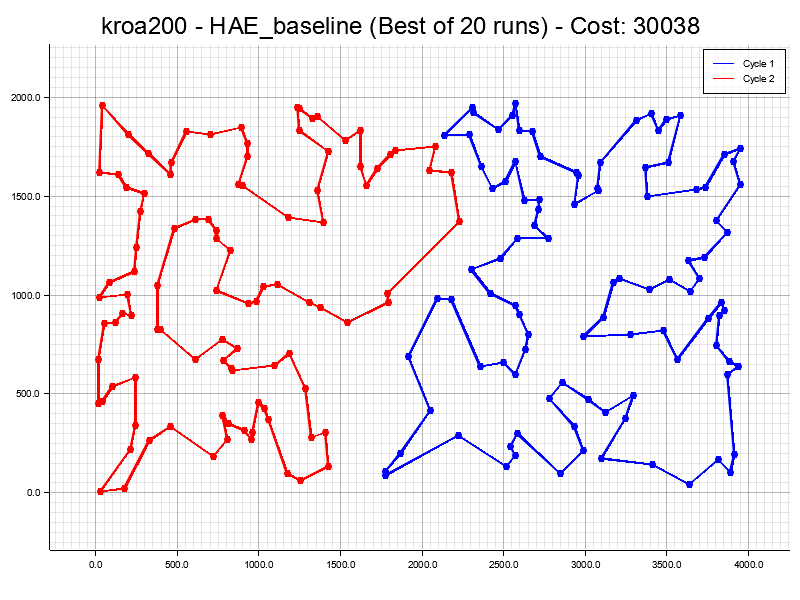
\includegraphics[width=\textwidth]{output/lab7/kroa200_HAE_baseline_best.png}
        \caption{kroa200 - HAE Baseline (najlepszy z 20)}
        \label{fig:kroa200_hae}
    \end{subfigure}
    \hfill
    \begin{subfigure}[b]{0.49\textwidth}
        \centering
        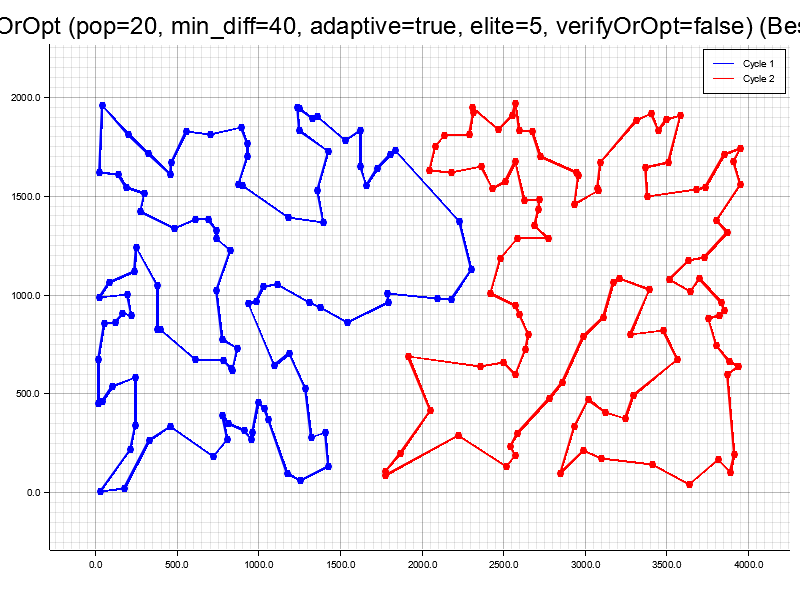
\includegraphics[width=\textwidth]{output/lab7/kroa200_EnhancedHAEOrOpt_best.png}
        \caption{kroa200 - EnhancedHaeOrOpt (najlepszy z 20)}
        \label{fig:kroa200_enhanced}
    \end{subfigure}
    \caption{Porównanie wizualizacji najlepszych rozwiązań dla instancji kroa200.}
    \label{fig:kroa200_comparison}
\end{adjustwidth}
\end{figure}

\begin{figure}[H]
\begin{adjustwidth}{-1cm}{-1cm}
    \centering
    \begin{subfigure}[b]{0.49\textwidth}
        \centering
        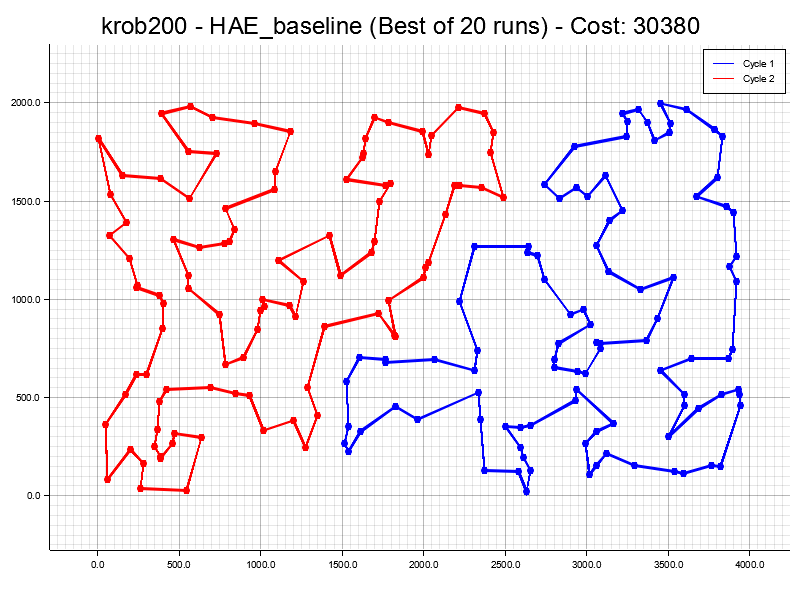
\includegraphics[width=\textwidth]{output/lab7/krob200_HAE_baseline_best.png}
        \caption{krob200 - HAE Baseline (najlepszy z 20)}
        \label{fig:krob200_hae}
    \end{subfigure}
    \hfill
    \begin{subfigure}[b]{0.49\textwidth}
        \centering
        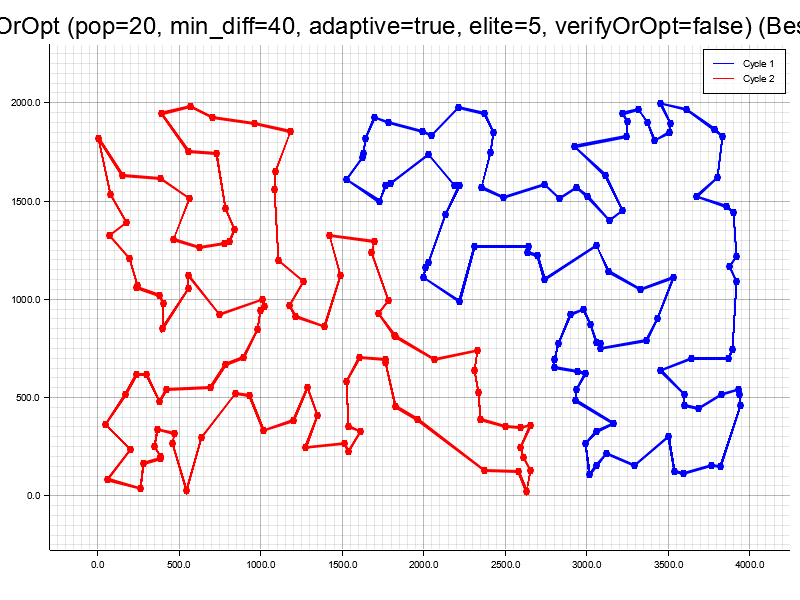
\includegraphics[width=\textwidth]{output/lab7/krob200_EnhancedHAEOrOpt_best.png}
        \caption{krob200 - EnhancedHaeOrOpt (najlepszy z 20)}
        \label{fig:krob200_enhanced}
    \end{subfigure}
    \caption{Porównanie wizualizacji najlepszych rozwiązań dla instancji krob200.}
    \label{fig:krob200_comparison}
\end{adjustwidth}
\end{figure}

\section{Wnioski Ogólne}
% Wnioski zostaną zaktualizowane na końcu
Analiza globalnej wypukłości (Laboratorium 6) dostarczyła wglądu w strukturę przestrzeni rozwiązań problemu 2-TSP. Zaobserwowane korelacje, zwłaszcza dla miary wspólnych krawędzi, sugerują, że rozwiązania o niższym koszcie wykazują pewne podobieństwa strukturalne. Stwierdzenie to, w połączeniu z obserwacją, że prawdopodobnie istnieje wiele dobrych, lecz strukturalnie odmiennych od siebie optimów lokalnych, potwierdziło zasadność stosowania algorytmów opartych na populacji oraz intensywnego przeszukiwania lokalnego, które są w stanie efektywnie eksplorować złożone przestrzenie rozwiązań.

Zaprojektowany w ramach Laboratorium 7 algorytm `EnhancedHaeOrOpt` okazał się skuteczny, przynosząc statystycznie istotną poprawę w jakości znajdowanych rozwiązań w porównaniu do bazowej wersji HAE. Kluczowe dla sukcesu było wprowadzenie operatora Or-Opt oraz adaptacyjny wybór operatorów lokalnego przeszukiwania. Ulepszone mechanizmy rekombinacji, inicjalizacji populacji i dywersyfikacji również przyczyniły się do lepszej eksploracji przestrzeni rozwiązań. Średnia poprawa rzędu +1.51\% dla kroa200 i +2.41\% dla krob200 (przy 20 uruchomieniach) potwierdza przewagę nowego algorytmu.

Możliwe kierunki dalszych badań obejmują testowanie innych zaawansowanych operatorów (np. 3-Opt), dokładniejszą analizę i strojenie parametrów algorytmu, oraz badanie wpływu różnych strategii dywersyfikacji i adaptacji na jeszcze bardziej złożonych instancjach problemu.

\section{Kod źródłowy}
Pełny kod źródłowy implementacji wszystkich algorytmów jest dostępny w repozytorium GitHub:
\url{https://github.com/Veanir/imo-7}

\end{document} 